\documentclass{article}

\usepackage{tikz}
\usetikzlibrary{graphs}
\usetikzlibrary{graphs.standard}
\usetikzlibrary{decorations.markings}
\usetikzlibrary{fit}
\usepackage{tikz-3dplot}
\usepackage{intcalc} %intcalcMod{r}{n} modular arithmetic (r mod n)
\usepackage{ifthen} % Allows boolean operations and if then else statements
\usepackage{amsfonts} % R, C, Z, Q,...

% Place good looking vertex. Syntax: \vertex{label}{x-coord,y-coord}
\newcommand*{\vertex}[2]{
	\node[circle, inner sep = 2pt, draw=black, fill=black] (#1) at #2 {};
}

\newcommand\R{\mathbb{R}}
\newcommand\C{\mathbb{C}}

\title{Some Automatically Created Graphs with Ti\textit{k}Z\\\vspace{10pt}See source code to change number of vertices in each graph}
\author{Gerald Todd\\University of Montana}

\begin{document}

\maketitle

\vspace{50pt}


%--------------COMPLETE BIPARTITE------------------------

% SET PARTITION SIZE HERE
\def\biparsize{10}

% Label
$$K_{\biparsize,\biparsize}$$\\

\begin{tikzpicture}

	\centering

	% Draws grid
	\pgfmathtruncatemacro\gridsize{\biparsize+1}
	\draw [help lines] (0,-5) grid (\gridsize,1);

	% Places vertices
	% Looping through vertex in first partition
	\foreach \cnt in {1,...,\biparsize} {
		
		% Generating label numbers for vertices in the second partition
		\pgfmathtruncatemacro\nextcnt{\cnt+\biparsize}
		
		% Placing vertices in first partition
		\vertex{\cnt}{(\cnt,0)};
		
		% Placing vertices in second partition
		\vertex{\nextcnt}{(\cnt,-4)};
		}
		
	% Draws edges
	% Looping through each vertex in the first partition
	\foreach \topnode in {1,...,\biparsize} {
	
		% Looping through each vertex in first partition again
		\foreach \lowstart in {1,...,\biparsize} {
			
			% Shifting one set of vertices so they now are in the second partition
			\pgfmathtruncatemacro\lownode{\lowstart+\biparsize}
			
			% Drawing edges between the sets
			\draw (\topnode)--(\lownode);
		}
	}
	

\end{tikzpicture}\\

\tikz[x=4cm] \graph[nodes={circle,fill,draw,inner sep=2pt}, empty nodes] {
	subgraph K_nm [V={1,...,10},W={11,...,20}]
};


\clearpage


%-----------------CIRCULAR COMPLETE---------------------

% SET GRAPH SIZE HERE
\def\size{35}

% Label
$$K_{\size}$$\\

\begin{tikzpicture}

	\centering

	% Places vertices evenly on radius
	% Looping though each vertex number
	\foreach \cnt in {1,...,\size} {
		
		% Placing each vertex evenly. ':' represents use of polar coordinates. i.e. (angle:radius)
		\vertex{\cnt}{(\cnt*360/\size:5)};
	}
		
	% Draws edges
	% Looping through each vertex where an edge starts
	\foreach \up in {1,...,\size} {
	
		% Looping through each vertex where an edge will terminate
		\foreach \low in {1,...,\size} {
		
			% Drawing each edge
			\draw (\up)--(\low);
		}
	}

\end{tikzpicture}

\tikz \graph[nodes={circle,draw,fill,inner sep=2pt},empty nodes] {subgraph K_n [clockwise, n=20,radius=4cm]};

\clearpage



%--------------------COMPLETE R-PARTITE ON N VERTS-------------------

% SET PARTITION NUMBER AND SIZE HERE
\def\parnum{5}
\def\parsize{2}

% Label
$$K_{\parsize}^{\parnum}$$\\

\begin{tikzpicture}

	\centering

	% Places nodes
	% Looping through each partition
	\foreach \part in {1,...,\parnum} {
	
		% Rotate to k*360/r degrees
		\begin{scope}[rotate=\part*360/\parnum]
		
		% Generating v_1 through v_n
		\foreach \vertstart in {1,...,\parsize} {
		
			% Shifting those vertices to their correct partition (v_{1+k*n} through v_{n+k*n})
			\pgfmathtruncatemacro\vert{\vertstart+(\part-1)*\parsize}
			
			 % Placing each vertex (shifted down so symmetric about x-axis), and naming them in order (1 though r*n) 
			\vertex{\vert}{(6,\vertstart-\parsize/2-.5)};
		}
		\end{scope}
	}
	
	% Draws edges
	% After drawing edges from the first r-1 paritions, all edges are present, so only consider r-1 partitions.
	\pgfmathtruncatemacro\lessparnum{\parnum-1}
	
	% Looping through the first r-1 partitions
	\foreach \part in {1,...,\lessparnum} {
	
		% Looping through each vertex in the first partition
		\foreach \vert in {1,...,\parsize} {
		
			% Shifting it to the appropriate vertex in the kth partition
			\pgfmathtruncatemacro\startvert{\vert+(\part-1)*\parsize}
			
			% Calculating the number of vertices not in the kth partition (we will draw edges to these)
			\pgfmathtruncatemacro\restparsize{\parsize*(\parnum-1)}
			
			% Looping through each of the vertices not in the kth parition
			\foreach \vertt in {1,...,\restparsize} {
			
				% Boolean condition determining the vertex where each edge ends
				\ifthenelse{ % if
					% We don't want to call vertex (0), it doesn't exist. So, if we are on v_{r*n},
					% \intcalcMod{}{}=0, so output r*n instead. Otherwise, just calculate the number
					% mod r*n
					\intcalcMod{\part*\parsize+\vertt}{\parsize*\parnum}=0}{ % then
					\pgfmathtruncatemacro\endvert{\parsize*\parnum}}{ % else
					\pgfmathtruncatemacro\endvert{\intcalcMod{\part*\parsize+\vertt}{\parsize*\parnum}}
				}
				
				% Drawing each edge
				\draw (\startvert)--(\endvert);
			}
		}
	}
	
	
\end{tikzpicture}

\clearpage


%------------------------HIGH MINIMUM DEGREE AND CUT VERTEX----------------------------


\center{A graph with high minimum degree and a cut vertex\\\vspace{10pt}(Example of rotating components who are themselves generated by rotations)}\vspace{20pt}

%-----DETERMINE THE NUMBER OF COMPONENTS HERE--------
\newcommand\parts{9}

% Define new function that creates a K^n with syntax \kx{n}
\newcommand\kx[1]{
	
	% Shifting index
	\pgfmathtruncatemacro\index{#1-1}
	% for loop that indexes the vertices
	\foreach \x in {0,...,\index} {
		%Determining parity of |G|
		\ifthenelse{\isodd{#1}}
			%Odd graphs get an extra rotation of (180/n) so a vertex will lie on the extreme left
			{\pgfmathtruncatemacro\angle{\x*(360/#1)-180/#1}}
			{\pgfmathtruncatemacro\angle{\x*(360/#1)}}
		%Placing each vertex
		\vertex{\x}{(\angle:1.5)};
	}
	
	% for loop that indexes the vertices
	\foreach \x in {0,...,\index} {
		% another loop that indexes the remaining vertices
		\foreach \y in {1,...,\index} {
			% mod arithmetic, e.g. for K^5, changing vertex 6 to vertex 1
			\pgfmathtruncatemacro\end{\intcalcMod{\x+\y}{#1}}
			% Drawing the edges
			\draw (\x)--(\end);
		}

	}
}
% End new function


\begin{tikzpicture}
	
	% Shifting index
	\pgfmathtruncatemacro\index{\parts-1}
	% for loop indexing the complete parts
	\foreach \x in {0,...,\index} {
		% Taking each complete graph, shifting it 120pts to the right, and rotating k*360/n degrees
		\begin{scope}[rotate=\x*360/\parts, xshift=120]
			\kx{\parts};
		\end{scope}
	}
	
	% Center vertex
	\vertex{}{(0,0)};
	
	% for loop indexing the complete parts
	\foreach \x in {0,...,\index} {
		% Drawing n horizontal edges and rotating each one the appropriate amount
		\begin{scope}[rotate=\x*(360/\parts)]
			\draw (0,0)--(81pt,0);
		\end{scope}
	}
	
\end{tikzpicture}


\clearpage


%--------------MINIMUM DEGREE n-1 AND NO HAMILTON PATH----------

\center{A graph with minimum degree $\displaystyle \frac{n-1}{2}$ but no Hamilton path}\vspace{20pt}

\newcommand\n{12}

\begin{tikzpicture}[scale=2]

	\ifthenelse{\isodd{\n}} {
		\begin{scope}[rotate=180/\n]
			\kx{\n};
		\end{scope}
	} {
		\kx{\n};
	}
	
	\begin{scope}[xshift=85.3]
		\kx{\n};
	\end{scope}
	
\end{tikzpicture}
	
\clearpage

%----------------------DRAWING SOME FUNCTIONS-------------------

\center{Some Functions}\\
\vspace{10pt}

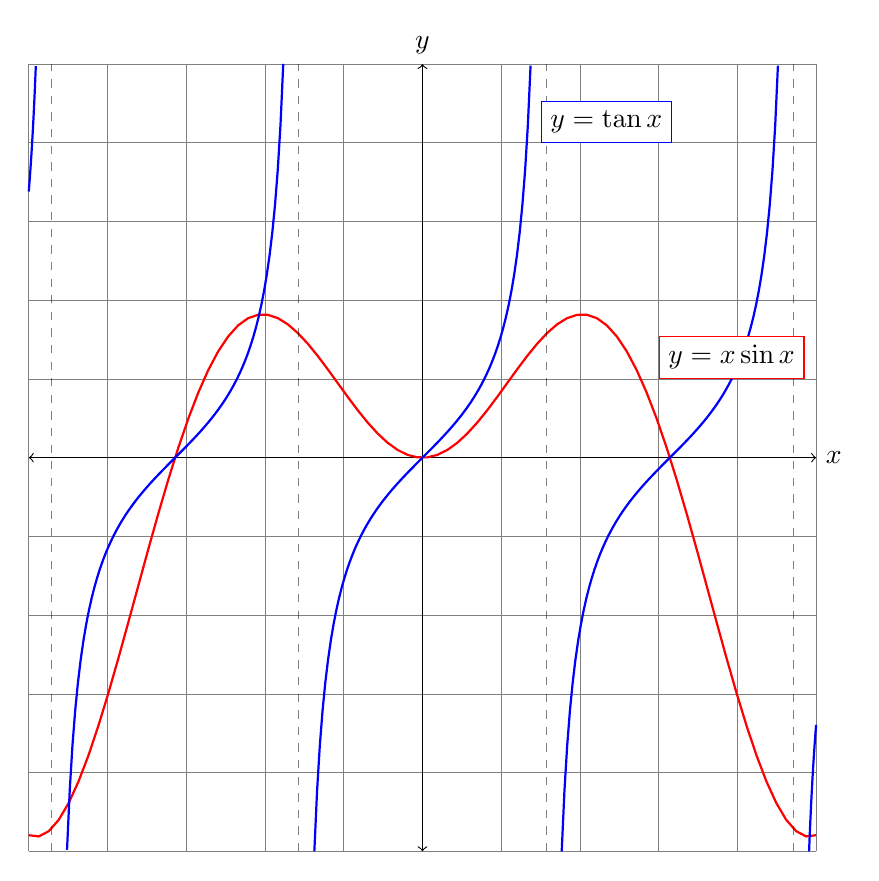
\begin{tikzpicture}

	% Drawing and labeling plane
	\draw [help lines] (-5,-5) grid (5,5);
	\draw [<->] (-5,0)--(5,0);
	\draw [<->] (0,-5)--(0,5);
	\node [right] at (5,0) {$x$};
	\node [above] at (0,5) {$y$};
	
	%Plotting xsinx
	\draw [red, thick, domain=-5:5, samples=80] plot (\x, {\x*sin(\x r)});
	
	%Plotting tanx
	\draw [blue, thick, domain=-1.3734:1.3734, samples=80] plot (\x, {tan(\x r)});
	\draw [blue, thick, domain=1.76819:4.51499, samples=80] plot (\x, {tan(\x r)});
	\draw [blue, thick, domain=-1.76819:-4.51499, samples=80] plot (\x, {tan(\x r)});
	\draw [blue, thick, domain=4.9098:5, samples=80] plot (\x, {tan(\x r)});
	\draw [blue, thick, domain=-5:-4.9098, samples=80] plot (\x, {tan(\x r)});
	
	%Plotting asymptotes
	\draw[dashed, opacity=.5] (-1.5708,-5)--(-1.5708,5);
	\draw[dashed, opacity=.5] (1.5708,-5)--(1.5708,5);
	\draw[dashed, opacity=.5] (-4.7124,-5)--(-4.7124,5);
	\draw[dashed, opacity=.5] (4.7124,-5)--(4.7124,5);
	
	%Labelling
	\node [above right, draw=red, fill=white] at (3,1){$y=x\sin x$};
	\node [above right, draw=blue, fill=white] at (1.5,4){$y=\tan x$};
	
\end{tikzpicture}


\clearpage


\center{Approximating $f(x)=e^x$ with a partial Taylor Series, $\displaystyle \sum_{k=0}^n\frac{x^n}{n!}$.}\\

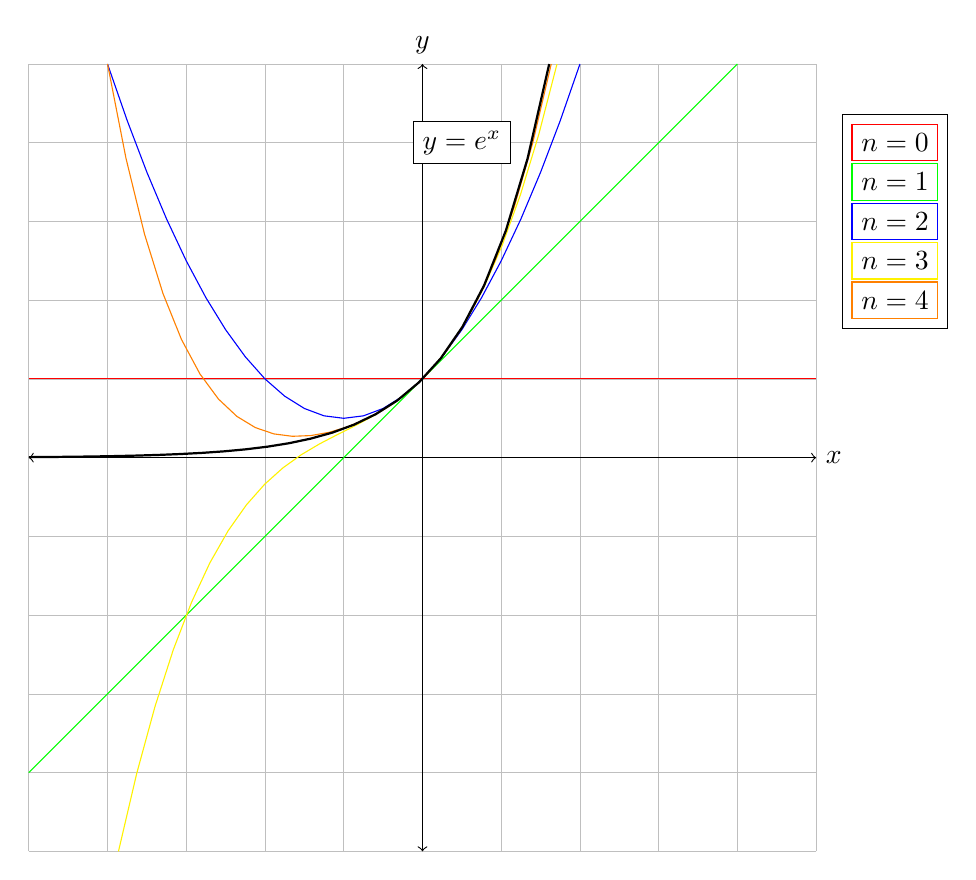
\begin{tikzpicture}

	%Drawing and labelling the plane
	\draw [help lines,opacity=.5] (-5,-5) grid (5,5);
	\draw[<->] (-5,0)--(5,0);
	\draw[<->] (0,-5)--(0,5);
	\node[right] at (5,0) {$x$};
	\node[above] at (0,5) {$y$};
	
	\draw [red, domain=-5:5] plot (\x,{1});
	\draw [green, domain=-5:4] plot (\x,{1+\x});
	\draw [blue, domain=-4:2] plot (\x,{1+\x+(\x)^2 /2});
	\draw [yellow, domain=-3.861:1.7087] plot (\x,{1+\x +(\x)^2 /2+ (\x)^3 /6});
	\draw [orange, domain=-4:1.6355] plot (\x,{1 +\x + (\x)^2 /2 + (\x)^3 /6 + (\x)^4 /24});
	\draw [black, thick, domain=-5:1.6094] plot (\x,{e^(\x)});
	
	\node [draw=red](r) at (6,4) {$n=0$};
	\node [draw=green](g) at (6,3.5) {$n=1$};
	\node [draw=blue](b) at (6,3) {$n=2$};
	\node [draw=yellow](y) at (6,2.5) {$n=3$};
	\node [draw=orange](o) at (6,2) {$n=4$};
	\node [fit=(r)(g)(b)(y)(o), draw] {};
	
	\node [draw, fill=white] at (.5,4) {$y=e^x$};
	

	
	
\end{tikzpicture}



\clearpage


\center{The Slit-Plane}\\
\vspace{10pt}

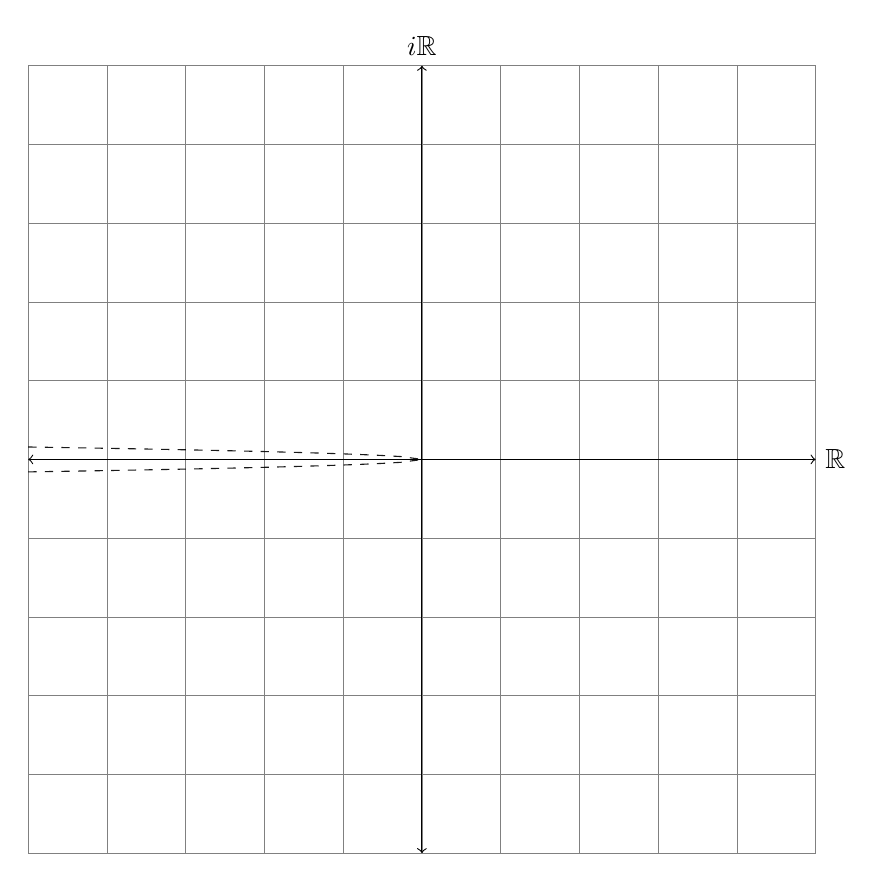
\begin{tikzpicture}

	% Drawing and labeling the complex plane
	\draw [help lines] (-5,-5) grid (5,5);
	\draw [<->] (-5,0)--(5,0);
	\draw [<->] (0,-5)--(0,5);
	\node [right] at (5,0) {$\R$};
	\node [above] at (0,5) {$i\R$};
	
	% Drawing slit
	\draw [dashed, opacity=.9, domain=-5:0, samples=20] plot (\x, {sqrt(-.5*\x)*.1});
	\draw [dashed, opacity=.9, domain=-5:0, samples=20] plot (\x, {-sqrt(-.5*\x)*.1});
	
\end{tikzpicture}


\clearpage

\center{Taken From the Internet\\Penrose Triangle}\vspace{10pt}

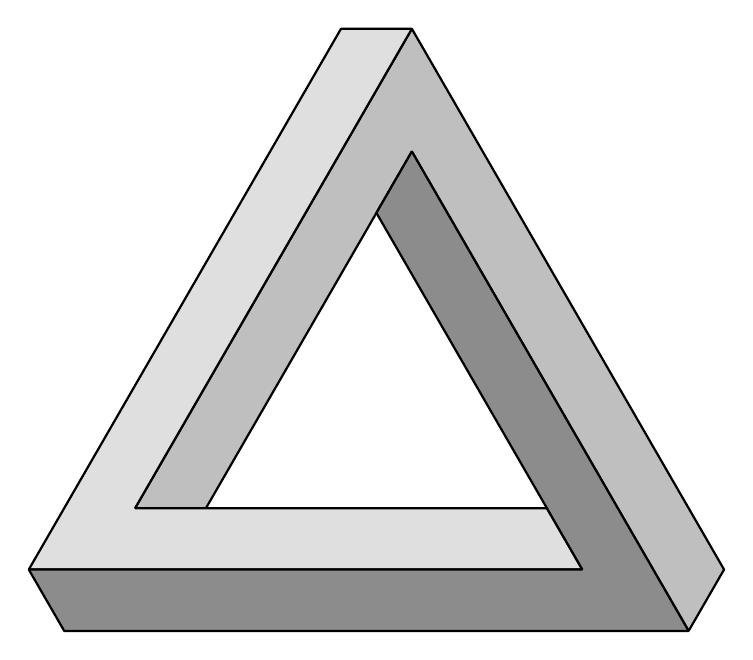
\begin{tikzpicture}[scale=1, line join=bevel]

	\centering
	
    % \a and \b are two macros defining characteristic
    % dimensions of the Penrose triangle.		
    \pgfmathsetmacro{\a}{2.5}
    \pgfmathsetmacro{\b}{0.9}

    \tikzset{%
      apply style/.code     = {\tikzset{#1}},
      triangle_edges/.style = {thick,draw=black}
    }

    \foreach \theta/\facestyle in {%
        0/{triangle_edges, fill = gray!50},
      120/{triangle_edges, fill = gray!25},
      240/{triangle_edges, fill = gray!90}%
    }{
      \begin{scope}[rotate=\theta]
        \draw[apply style/.expand once=\facestyle]
          ({-sqrt(3)/2*\a},{-0.5*\a})                     --
          ++(-\b,0)                                       --
            ({0.5*\b},{\a+3*sqrt(3)/2*\b})                -- % higher point	
            ({sqrt(3)/2*\a+2.5*\b},{-.5*\a-sqrt(3)/2*\b}) -- % rightmost point
          ++({-.5*\b},-{sqrt(3)/2*\b})                    -- % lower point
            ({0.5*\b},{\a+sqrt(3)/2*\b})                  --
          cycle;
        \end{scope}
      }	
	  \end{tikzpicture}



\clearpage


\tdplotsetmaincoords{70}{110}
\begin{tikzpicture}[scale=3,tdplot_main_coords]
    \draw[thick,->] (0,0,0) -- (1,0,0) node[anchor=north east]{$x$};
    \def\x{.5}
    \draw[thin] (0,0,0) -- ({1.2*\x},{sqrt(3)*1.2*\x},0) node[below] {$y=\sqrt{3}x$};
    \filldraw[
        draw=red,%
        fill=red!20,%
    ]          (0,0,0)
            -- (\x,{sqrt(3)*\x},0)
            -- (\x,{sqrt(3)*\x},1)
            -- (0,0,1)
            -- cycle;
    \draw[thick,->] (0,0,0) -- (0,1,0) node[anchor=north west]{$y$};
    \draw[thick,->] (0,0,0) -- (0,0,1) node[anchor=south]{$z$};
\end{tikzpicture}



\clearpage

% Unit circle
% Author: Supreme Aryal
% A unit circle with cosine and sine values for some
% common angles.


    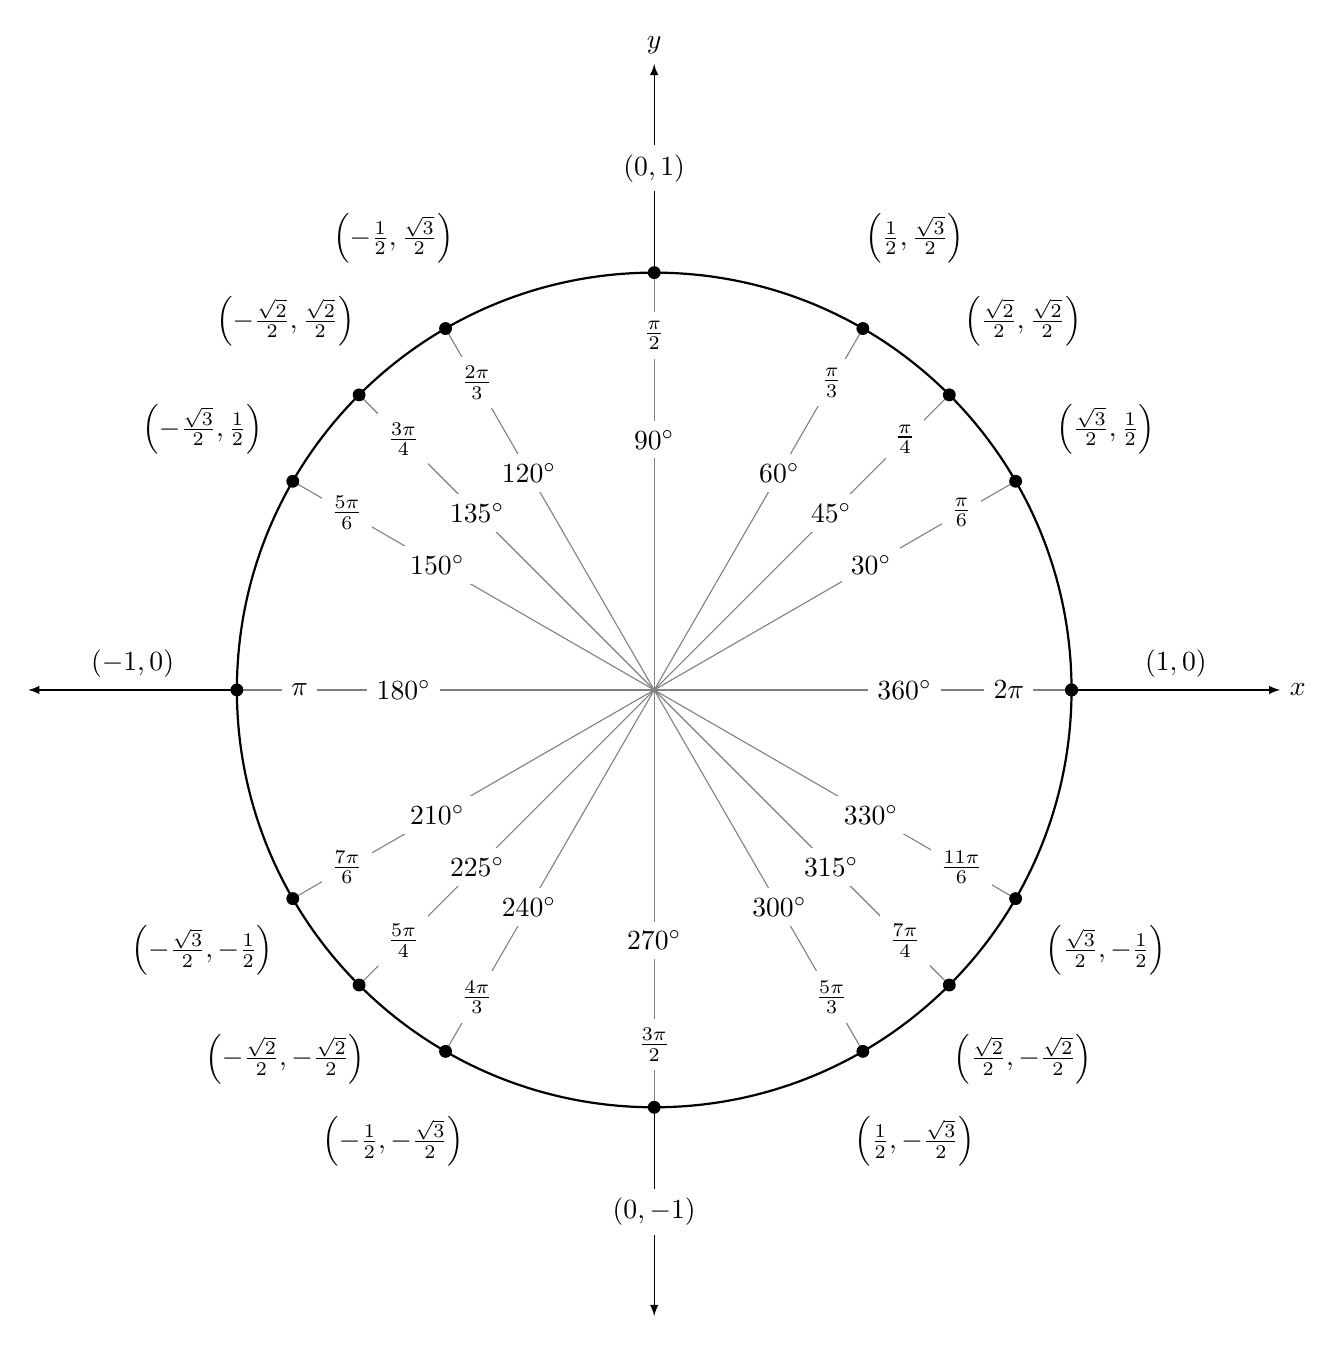
\begin{tikzpicture}[scale=5.3,cap=round,>=latex]
        % draw the coordinates
        \draw[<->] (-1.5cm,0cm) -- (1.5cm,0cm) node[right,fill=white] {$x$};
        \draw[<->] (0cm,-1.5cm) -- (0cm,1.5cm) node[above,fill=white] {$y$};

        % draw the unit circle
        \draw[thick] (0cm,0cm) circle(1cm);

        \foreach \x in {0,30,...,360} {
                % lines from center to point
                \draw[gray] (0cm,0cm) -- (\x:1cm);
                % dots at each point
                \filldraw[black] (\x:1cm) circle(0.4pt);
                % draw each angle in degrees
                \draw (\x:0.6cm) node[fill=white] {$\x^\circ$};
        }
        
       \foreach \x in {45,135,...,315} {
       		\draw[gray] (0,0)--(\x:1cm);
		\filldraw[black] (\x:1cm) circle(.4pt);
		\draw (\x:.6cm) node[fill=white] {$\x^\circ$};
	}

        % draw each angle in radians
        \foreach \x/\xtext in {
            30/\frac{\pi}{6},
            45/\frac{\pi}{4},
            60/\frac{\pi}{3},
            90/\frac{\pi}{2},
            120/\frac{2\pi}{3},
            135/\frac{3\pi}{4},
            150/\frac{5\pi}{6},
            180/\pi,
            210/\frac{7\pi}{6},
            225/\frac{5\pi}{4},
            240/\frac{4\pi}{3},
            270/\frac{3\pi}{2},
            300/\frac{5\pi}{3},
            315/\frac{7\pi}{4},
            330/\frac{11\pi}{6},
            360/2\pi}
                \draw (\x:0.85cm) node[fill=white] {$\xtext$};

        \foreach \x/\xtext/\y in {
            % the coordinates for the first quadrant
            30/\frac{\sqrt{3}}{2}/\frac{1}{2},
            45/\frac{\sqrt{2}}{2}/\frac{\sqrt{2}}{2},
            60/\frac{1}{2}/\frac{\sqrt{3}}{2},
            % the coordinates for the second quadrant
            150/-\frac{\sqrt{3}}{2}/\frac{1}{2},
            135/-\frac{\sqrt{2}}{2}/\frac{\sqrt{2}}{2},
            120/-\frac{1}{2}/\frac{\sqrt{3}}{2},
            % the coordinates for the third quadrant
            210/-\frac{\sqrt{3}}{2}/-\frac{1}{2},
            225/-\frac{\sqrt{2}}{2}/-\frac{\sqrt{2}}{2},
            240/-\frac{1}{2}/-\frac{\sqrt{3}}{2},
            % the coordinates for the fourth quadrant
            330/\frac{\sqrt{3}}{2}/-\frac{1}{2},
            315/\frac{\sqrt{2}}{2}/-\frac{\sqrt{2}}{2},
            300/\frac{1}{2}/-\frac{\sqrt{3}}{2}}
                \draw (\x:1.25cm) node[fill=white] {$\left(\xtext,\y\right)$};

        % draw the horizontal and vertical coordinates
        % the placement is better this way
        \draw (-1.25cm,0cm) node[above=1pt] {$(-1,0)$}
              (1.25cm,0cm)  node[above=1pt] {$(1,0)$}
              (0cm,-1.25cm) node[fill=white] {$(0,-1)$}
              (0cm,1.25cm)  node[fill=white] {$(0,1)$};
    \end{tikzpicture}
    

	
\end{document}









